\documentclass[a4paper,11pt]{article}
\usepackage{amsmath,amsthm,amsfonts,amssymb,amscd,amstext,vmargin,graphics,graphicx,tabularx,multicol} 
\usepackage[francais]{babel}
\usepackage[utf8]{inputenc}  
\usepackage[T1]{fontenc} 
\usepackage{pstricks-add,tikz,tkz-tab,variations}
\usepackage[autolanguage,np]{numprint} 
\usepackage{calc}

\setmarginsrb{1.5cm}{0.5cm}{1cm}{0.5cm}{0cm}{0cm}{0cm}{0cm} %Gauche, haut, droite, haut
\newcounter{numexo}
\newcommand{\exo}[1]{\stepcounter{numexo}\noindent{\bf Exercice~\thenumexo} : }
\reversemarginpar

\newcommand{\bmul}[1]{\begin{multicols}{#1}}
\newcommand{\emul}{\end{multicols}}

\newcounter{enumtabi}
\newcounter{enumtaba}
\newcommand{\q}{\stepcounter{enumtabi} \theenumtabi.  }
\newcommand{\qa}{\stepcounter{enumtaba} (\alph{enumtaba}) }
\newcommand{\initq}{\setcounter{enumtabi}{0}}
\newcommand{\initqa}{\setcounter{enumtaba}{0}}

\newcommand{\be}{\begin{enumerate}}
\newcommand{\ee}{\end{enumerate}}
\newcommand{\bi}{\begin{itemize}}
\newcommand{\ei}{\end{itemize}}
\newcommand{\bp}{\begin{pspicture*}}
\newcommand{\ep}{\end{pspicture*}}
\newcommand{\bt}{\begin{tabular}}
\newcommand{\et}{\end{tabular}}
\renewcommand{\tabularxcolumn}[1]{>{\centering}m{#1}} %(colonne m{} centrée, au lieu de p par défault) 
\newcommand{\tnl}{\tabularnewline}

\newcommand{\trait}{\noindent \rule{\linewidth}{0.2mm}}
\newcommand{\hs}[1]{\hspace{#1}}
\newcommand{\vs}[1]{\vspace{#1}}

\newcommand{\N}{\mathbb{N}}
\newcommand{\Z}{\mathbb{Z}}
\newcommand{\R}{\mathbb{R}}
\newcommand{\C}{\mathbb{C}}
\newcommand{\Dcal}{\mathcal{D}}
\newcommand{\Ccal}{\mathcal{C}}
\newcommand{\mc}{\mathcal}

\newcommand{\vect}[1]{\overrightarrow{#1}}
\newcommand{\ds}{\displaystyle}
\newcommand{\eq}{\quad \Leftrightarrow \quad}
\newcommand{\vecti}{\vec{\imath}}
\newcommand{\vectj}{\vec{\jmath}}
\newcommand{\Oij}{(O;\vec{\imath}, \vec{\jmath})}
\newcommand{\OIJ}{(O;I,J)}


\newcommand{\reponse}[1][1]{%
\multido{}{#1}{\makebox[\linewidth]{\rule[0pt]{0pt}{20pt}\dotfill}
}}

\newcommand{\titre}[5] 
% #1: titre #2: haut gauche #3: bas gauche #4: haut droite #5: bas droite
{
\noindent #2 \hfill #4 \\
#3 \hfill #5

\vspace{-1.6cm}

\begin{center}\rule{6cm}{0.5mm}\end{center}
\vspace{0.2cm}
\begin{center}{\large{\textbf{#1}}}\end{center}
\begin{center}\rule{6cm}{0.5mm}\end{center}
}



\begin{document}
\pagestyle{empty}
\titre{Séance d'AP  : Calculs de volumes}{}{}{3ème}{}




\exo\\
\bmul{2}
Sur un parking, une commune veut regrouper 6 conteneurs à déchets du même modèle A ou B. Les deux modèles sont fabriqués dans le même matériau qui a partout la même épaisseur.\\

\bi
\item Le conteneur A est un pavé droit à base carrée de côté 1 m, et de hauteur 2 m  ;
 \item le conteneur B est constitué de 2 demi-sphères de rayon 0,58 m et d'un cylindre de même rayon et de hauteur 1,15 m.

\ei

\columnbreak


\begin{center}
\includegraphics[scale=0.8]{volap3.eps} 
\end{center}

\emul

 Vérifier que les 2 conteneurs ont pratiquement le même volume. \\


\vspace*{0.5cm}

\exo\\
Le culbuto ci-contre est un jouet pour enfant qui oscille sur une base sphérique. 

\bmul{2}

\initqa \qa Calculer son volume exact puis en donner l'arrondi au $cm^{3}$.\\


\qa On souhaite peindre en rouge la base sphérique. Calculer l'aire de la surface à peindre.\\ 
En donner la valeur exacte, puis l'arrondi au $cm^{2}$.\\

\qa Sachant que 1 L de peinture peut couvrir 5,5 $m^{2}$, combien de culbutos pourra-t-on mettre en peinture avec un pot de 2,5 L ?\\

\columnbreak

\begin{center}
\includegraphics[scale=0.8]{volap2..eps} 
\end{center}



\emul


\vspace*{0.5cm}


\exo\\
Une maison est composée d'une partie principale qui a la forme d'un pavé droit ABCDEFGH surmonté d'une pyramide IABCD de sommet I et de hauteur [IK1] perpendiculaire à la base de la pyramide.\\

Cette pyramide est coupée en deux parties :\\
- une partie basse ABCDRTSM destinée aux chambres ;\\
- une partie haute IRTSM réduction de hauteur [IK2] de la pyramide IABCD correspondant au grenier.\\

On a : EH = 12 m ; AE = 3 m ; HG = 9 m ; IK1 = 6,75 m et IK2 = 4,5 m.\\
\textit{La figure donnée n'est pas à l'échelle.}

\begin{center}
\includegraphics[scale=0.7]{brevtexo.eps} 
\end{center}

\initq \q Calculer la surface au sol de la maison.\\

\q Des radiateurs électriques seront installés dans toute la maison, excepté au grenier. On cherche le volume à chauffer de la maison.\\
On rappelle que le volume d'une pyramide est donné par : $ V = \dfrac{B \times h }{3} $\\

\initqa \qa Calculer le volume de la partie principale.\\

\qa Calculer le volume des chambres.\\

\qa Montrer que le volume à chauffer est égal à 495 $m^{3}$.\\

\q Un expert a estimé qu'il faut dans cette maison une puissance électrique de 925 watts pour chauffer 25 mètres cubes.\\
Le propriétaire de la maison décide d'acheter des radiateurs qui ont une puissance de 1 800 watts chacun et qui coûtent 349,90 euros pièce.\\
\hspace*{1.5cm} Combien va-t-il devoir dépenser pour l'achat des radiateurs ?\\

\vspace*{0.5cm}



\end{document}
